% run: lualatex abd-2am-latency-boxplot-stat.tex to avoid ``Tex capacity exceeded'' error
\documentclass{standalone}
\usepackage{pgfplots}
\usepackage{pgfplotstable}
\usepgfplotslibrary{groupplots}
\usepgfplotslibrary{statistics}

\pgfplotsset{ compat=1.8, }

\newcommand{\boxplottable}[8]{
  \addplot+[
    mark=x,
    boxplot prepared={
      draw position=#8,
      lower whisker=#1,
      lower quartile=#2,
      median=#3,
      upper quartile=#4,
      upper whisker=#5,
      average=#6,
      box extend=1.0,
      every whisker/.style={blue},
      every median/.style={densely dashed,cyan,thick},
      every average/.style={red,mark=10-pointed star},
    },
  ]
  coordinates {};
  %table[y index=0] {#7};
}

\newcommand{\boxplottablewithlabels}[7]{
  \addplot+[
    mark=x,
    boxplot prepared={
      lower whisker=#1,
      lower quartile=#2,
      median=#3,
      upper quartile=#4,
      upper whisker=#5,
      average=#6,
    },
  ]
  table[y index=0] {#7}
  [right]
  node at
  (boxplot box cs: \boxplotvalue{lower whisker},0)
  {\pgfmathprintnumber{\boxplotvalue{lower whisker}}}
  node at
  (boxplot box cs: \boxplotvalue{lower quartile},0)
  {\pgfmathprintnumber{\boxplotvalue{lower quartile}}}
  node[left] at
  (boxplot box cs: \boxplotvalue{median},0.4)
  {\pgfmathprintnumber{\boxplotvalue{median}}}
  node at
  (boxplot box cs: \boxplotvalue{upper quartile},0)
  {\pgfmathprintnumber{\boxplotvalue{upper quartile}}}
  node at
  (boxplot box cs: \boxplotvalue{upper whisker},0)
  {\pgfmathprintnumber{\boxplotvalue{upper whisker}}}
  node[right] at
  (boxplot box cs: \boxplotvalue{average},0.5)
  {\pgfmathprintnumber{\boxplotvalue{average}}}
  ;
}

\begin{document}
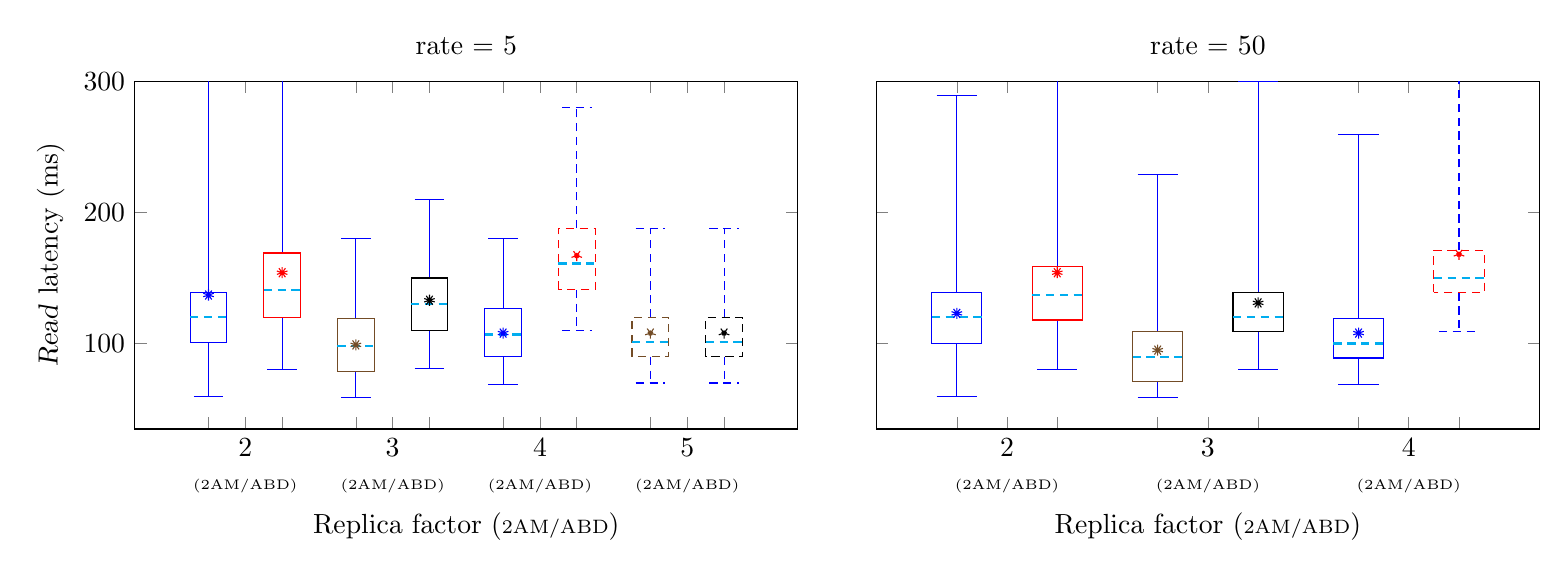
\begin{tikzpicture}
  \begin{groupplot}[
        group style={
	  group size=2 by 1,
	  y descriptions at=edge left,
	  x descriptions at=edge bottom,
	  horizontal sep=1.0cm,
	},
	boxplot/draw direction=y,
	% xtick={0.5,1.0,1.5, 2.5,3.0,3.5, 4.5,5.0,5.5, 6.5,7.0,7.5},
	xtick={1,2,3, 5,6,7, 9,10,11, 13,14,15},
	xticklabels={
	  {}, 
	  {2\\{\tiny (2AM/ABD)}},
	  {},
	  {},
	  {3\\{\tiny (2AM/ABD)}},
	  {},
	  {},
	  {4\\{\tiny (2AM/ABD)}},
	  {},
	  {},
	  {5\\{\tiny (2AM/ABD)}},
	  },
	x tick label style={
	    align=center,
	},
	ymax=300,
	skip coords between index={0}{5},
	xlabel={Replica factor ({\scriptsize 2AM/ABD})},
	ylabel={\textsl{Read} latency (ms)},
	height=6cm,
	width=10cm,
      ]

      \nextgroupplot[title={rate = $5$}]
      \boxplottable{60}{101}{120}{139}{631}{137}{boxplot-rate5-replica2-2am.txt}{1.0} % check it
      \boxplottable{80}{120}{141}{169}{321}{154}{boxplot-rate5-replica2-abd.txt}{3.0} % check it

      \boxplottable{59}{79}{98}{119}{180}{99}{boxplot-rate5-replica3-2am.txt}{5.0}
      \boxplottable{81}{110}{130}{150}{210}{133}{boxplot-rate5-replica3-abd.txt}{7.0}

      \boxplottable{69}{90}{107}{127}{180}{108}{boxplot-rate5-replica4-2am.txt}{9.0}
      \boxplottable{110}{141}{161}{188}{280}{167}{boxplot-rate5-replica4-abd.txt}{11.0}

      \boxplottable{70}{90}{101}{120}{188}{108}{boxplot-rate5-replica5-2am.txt}{13.0}
      \boxplottable{70}{90}{101}{120}{188}{108}{boxplot-rate5-replica5-2am.txt}{15.0} % using real data
    \nextgroupplot[title={rate = $50$}]
    \boxplottable{60}{100}{120}{139}{289}{123}{boxplot-rate50-replica2-2am.txt}{1.0}
    \boxplottable{80}{118}{137}{159}{700}{154}{boxplot-rate50-replica2-abd.txt}{3.0} % check it

    \boxplottable{59}{71}{90}{109}{229}{95}{boxplot-rate50-replica3-2am.txt}{5.0}
    \boxplottable{80}{109}{120}{139}{300}{131}{boxplot-rate50-replica3-abd.txt}{7.0}

    \boxplottable{69}{89}{100}{119}{259}{108}{boxplot-rate50-replica4-2am.txt}{9.0}
    \boxplottable{109}{139}{150}{171}{370}{168}{boxplot-rate50-replica4-abd.txt}{11.0}
      % replica=5
    \end{groupplot}
\end{tikzpicture}
\end{document}
